% Methodology
% Be specific enough that someone could reproduce your work

\label{sec:methodology}

% Overview
Using the Wikipedia API, we will track edits from frequently visited versions of Wikipedia for different countries for edits made by unregistered users. We will use the IP addresses of those unregistered users to link them to that editor’s country. This will be used to compare edit frequency per country against benchmarks for free speech laws. Our benchmarks for free speech laws will be sourced from the V-Dem democracy index.

\subsection{Data Collection}

We used the Wikipedia API for frequently visited versions of Wikipedia for different countries. The versions that we are focusing on are Wikipedia en (English), es (Spanish), ru (Russian), and hu (Hungarian). These versions of Wikipedia were selected based upon availability of unregistered user edits.

% Example of how to cite a dataset or tool:
% We collected data from the Wikipedia API \cite{wikipedia-api} covering...

\subsection{Data Processing}

We filtered out edits made by registered users, as we do not have access to their IP addresses. Unregistered user edits were linked to their respective country by IP address, as seen in Figure~\ref{fig:totaledits}. Our data processing pipeline is available in our GitHub repository.\footnote{\url{https://github.com/kochenderferc/wikipedia-political-context}} We then accounted for population size using the Rest Countries API.\footnote{\url{https://restcountries.com/}}

\begin{figure}
    \centering
    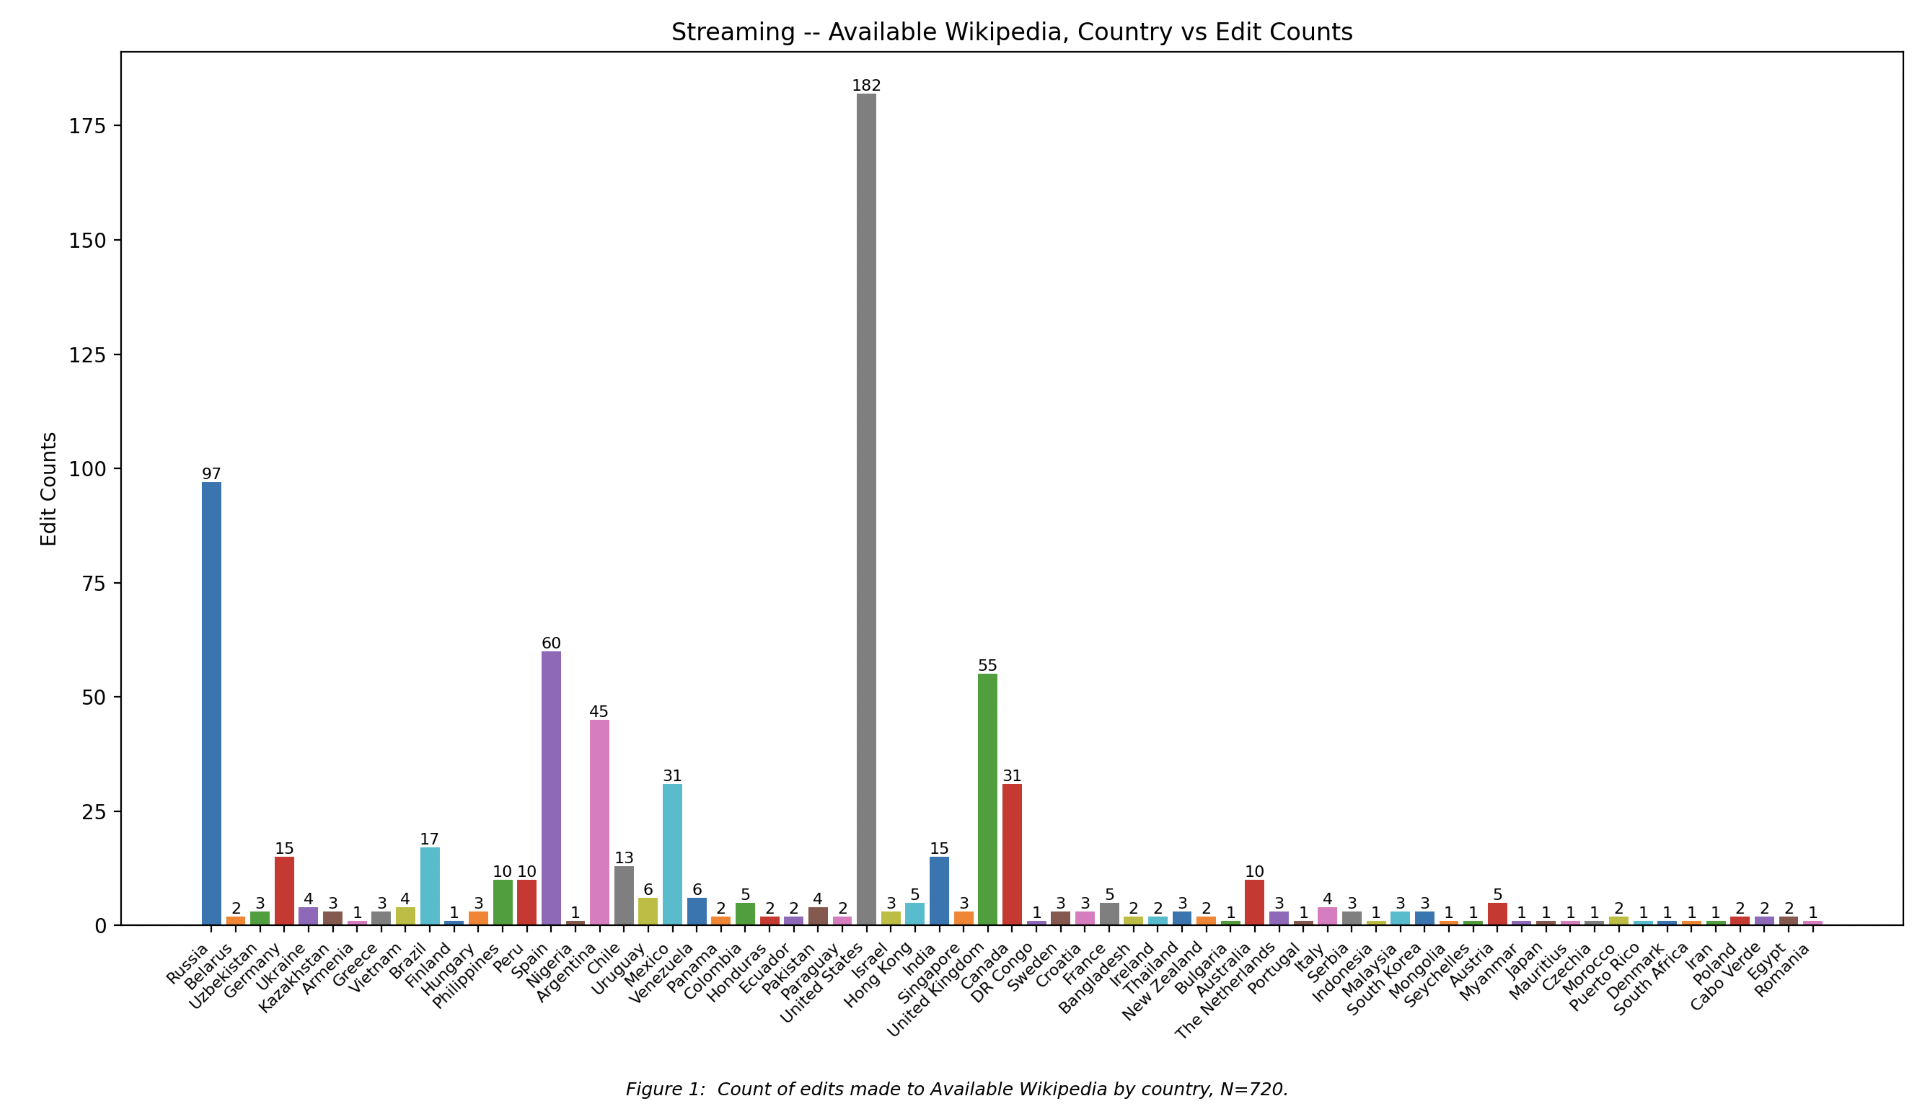
\includegraphics[width=\linewidth]{figures/totaledits.png}
    \caption{Unregistered Wikipedia edits per country}
    \label{fig:totaledits}
\end{figure}

\subsection{Analysis Methods}

We compared the results to the V-Dem (Varieties of Democracy) index to understand the link between freedom of speech and edits on Wikipedia. The relationship between liberal democracy and freedom of expression for 2023 is shown in Figure~\ref{fig:vdem}. This data for the selected Wikipedia countries was then overlaid with our data on unregistered edits, after accounting for population size. Our comparison prior to accounting for population size is shown in Figure~\ref{fig:initialcomparison}.

\begin{figure}
  \centering
  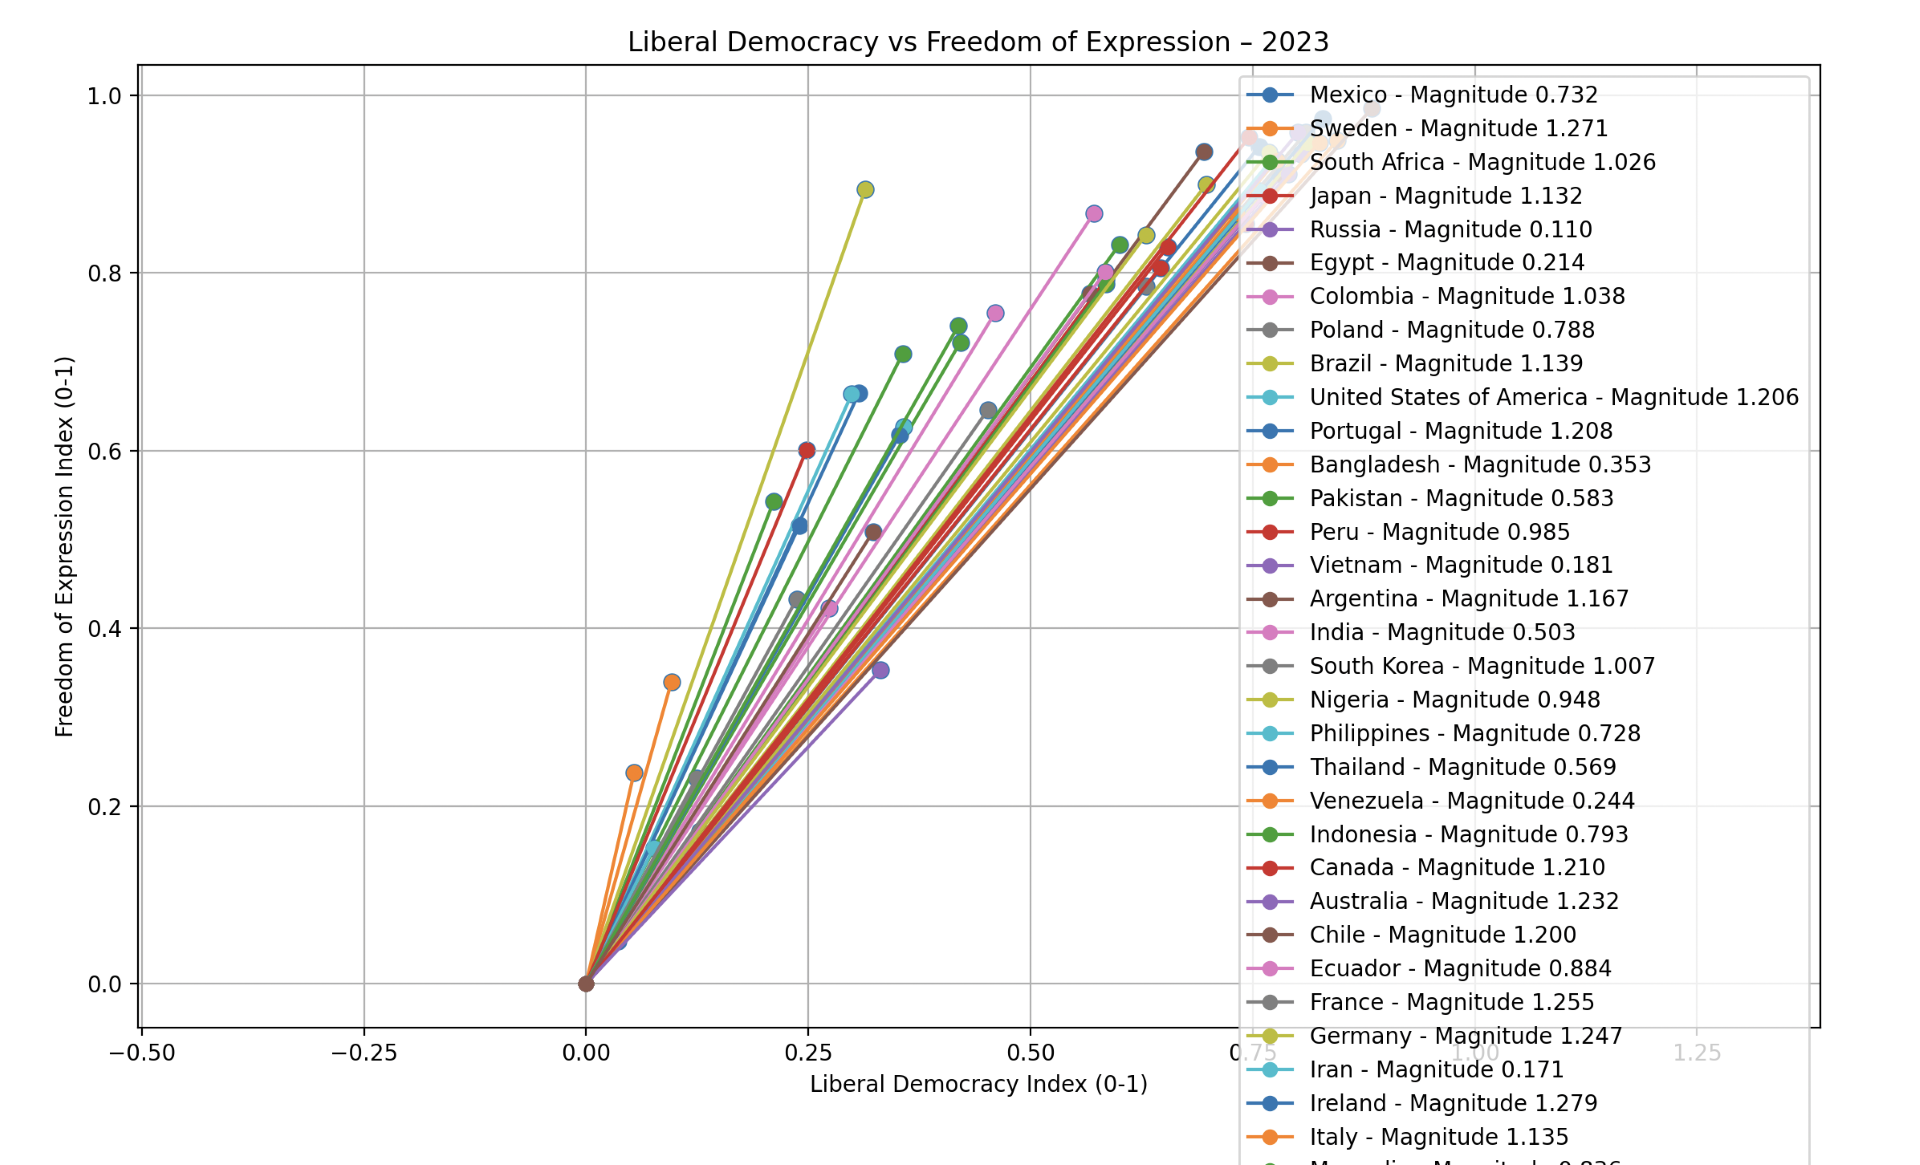
\includegraphics[width=\linewidth]{figures/vdem.png}
  \caption{Liberal Democracy vs. Freedom of Expression from the V-Dem index for 2023}
  \label{fig:vdem}
\end{figure}

\begin{figure}
    \centering
    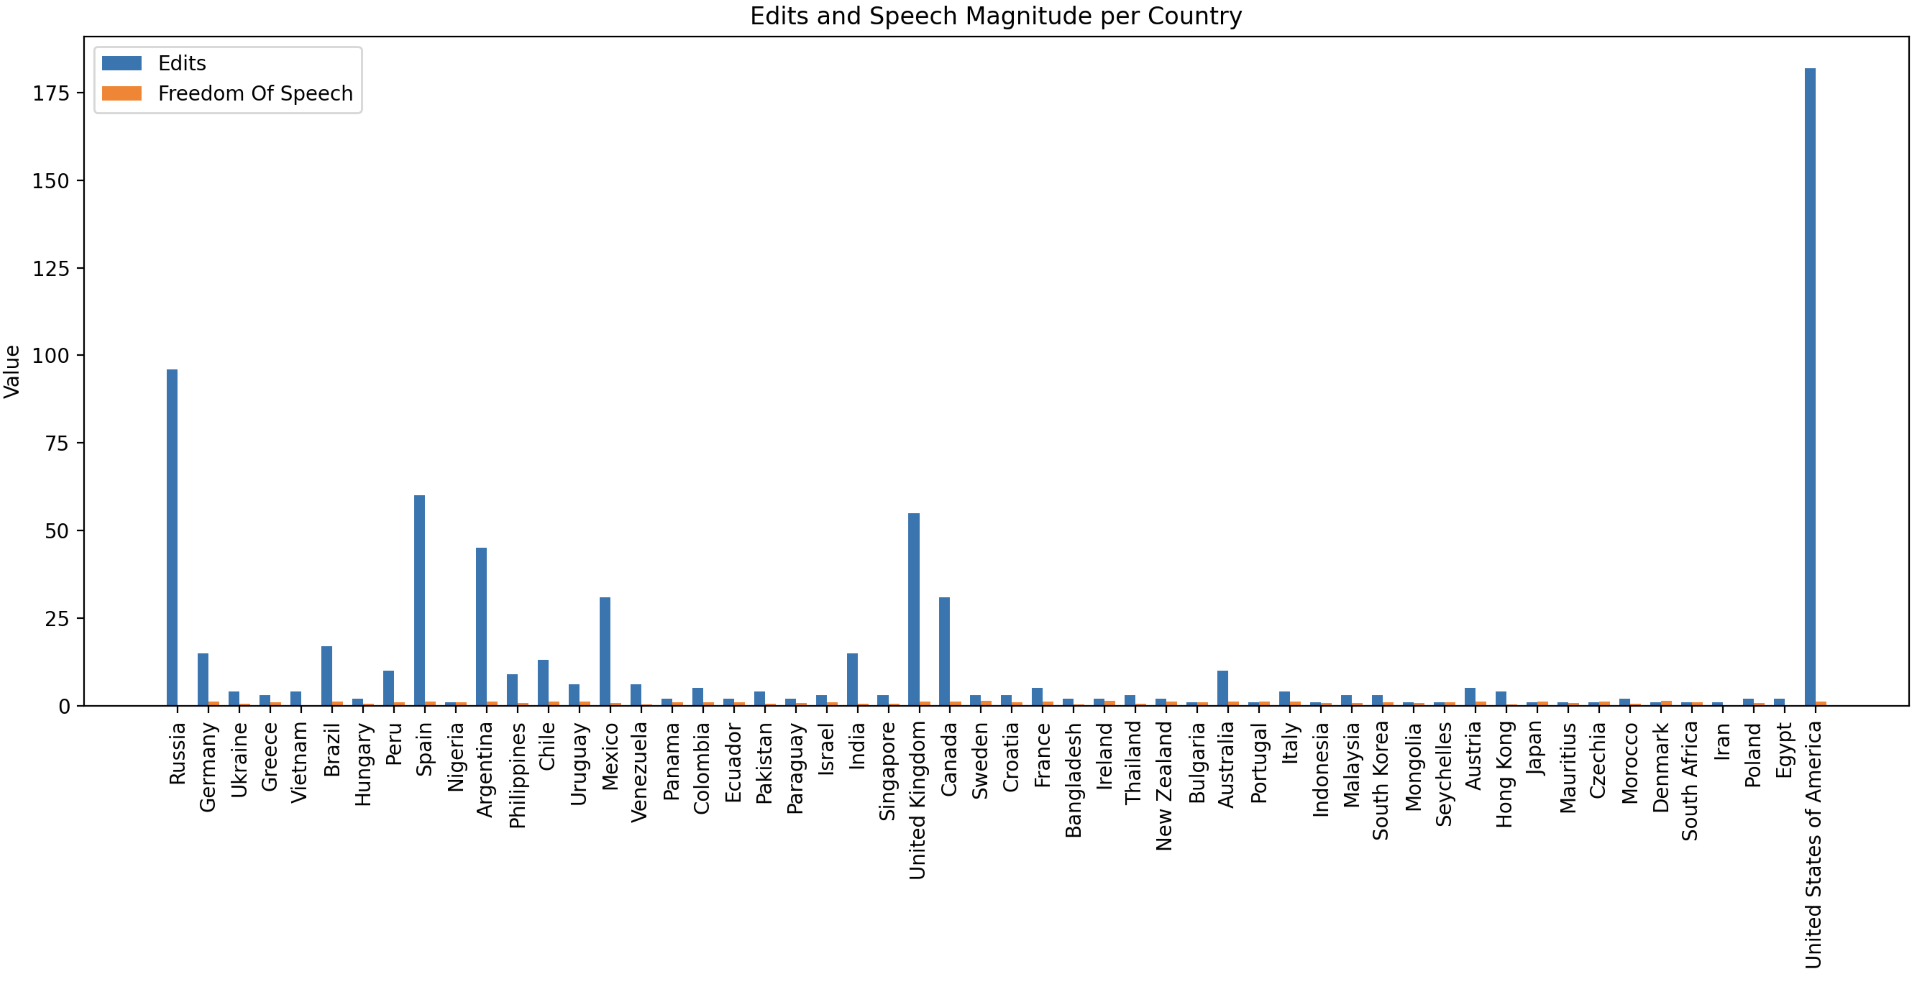
\includegraphics[width=\linewidth]{figures/initialcomparison.png}
    \caption{Initial comparison between unregistered edits and freedom of speech}
    \label{fig:initialcomparison}
\end{figure}

% If you have equations, you can include them:
% \begin{equation}
% your\_formula = here
% \end{equation}

\subsection{Ethical Considerations}
All data consists of publicly available Wikipedia content accessed in compliance with \href{https://foundation.wikimedia.org/wiki/Policy:Terms_of_Use}{Wikimedia's Terms of Use}.

